\documentclass[tikz,border=2pt]{standalone}

\usepackage{pgfplots}
\pgfplotsset{compat=1.18}

\begin{document}
	
	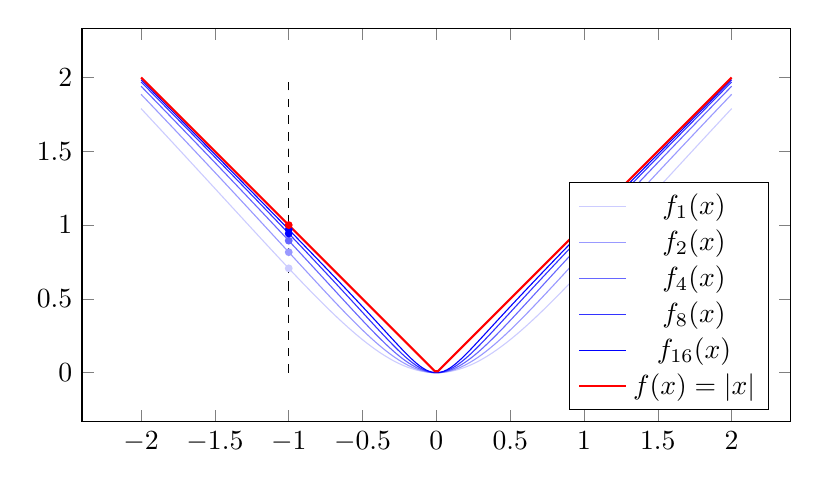
\begin{tikzpicture}
		\begin{axis}[
			axis equal,
			scale only axis,
			width=9cm,
			height=5cm,
			domain=-2:2,
			samples=200,
			no markers,
			legend pos=south east
			]
			\addplot[color=blue!20] ({x},{x^2/sqrt(x^2 + 1)});
			\addlegendentry{$f_1(x)$}
			
			\addplot[color=blue!40] ({x},{x^2/sqrt(x^2 + 1/2)});
			\addlegendentry{$f_2(x)$}
			
			\addplot[color=blue!60] ({x},{x^2/sqrt(x^2 + 1/4)});
			\addlegendentry{$f_4(x)$}
			
			\addplot[color=blue!80] ({x},{x^2/sqrt(x^2 + 1/8)});
			\addlegendentry{$f_8(x)$}
			
			\addplot[color=blue!100] ({x},{x^2/sqrt(x^2 + 1/16)});
			\addlegendentry{$f_{16}(x)$}
			
			\addplot[color=red, thick] ({x},{abs(x)});
			\addlegendentry{$f(x)=|x|$}
			
			\addplot[dashed, black, domain=0:2] (-1, x);
			\node[circle,fill,inner sep=1pt,color=blue!20] at (axis cs:-1,{1/sqrt(1 + 1)}) {};
			\node[circle,fill,inner sep=1pt,color=blue!40] at (axis cs:-1,{1/sqrt(1 + 1/2)}) {};
			\node[circle,fill,inner sep=1pt,color=blue!60] at (axis cs:-1,{1/sqrt(1 + 1/4)}) {};
			\node[circle,fill,inner sep=1pt,color=blue!100] at (axis cs:-1,{1/sqrt(1 + 1/8)}) {};
			\node[circle,fill,inner sep=1pt,color=blue!100] at (axis cs:-1,{1/sqrt(1 + 1/16)}) {};
			\node[circle,fill,inner sep=1pt,color=red] at (axis cs:-1,{1/sqrt(1)}) {};
		\end{axis}
	\end{tikzpicture}
	
\end{document}